% Time-stamp: <2022-11-08 07:39:29 A13258Q>
% Amine Raboun 2023, https://amineraboun.github.io/
% Romain Lafarguette 2023, https://romainlafarguette.github.io/

%% ---------------------------------------------------------------------------
%% Preamble: Packages and Setup
%% ---------------------------------------------------------------------------
% Class 
\documentclass{beamer}

% Theme
\usetheme{Boadilla}
\usecolortheme{dolphin}
%\setbeamertemplate{headline}{} % Remove the top navigation bar

% Font and encoding
\usepackage[utf8]{inputenc} % Input font
\usepackage[T1]{fontenc} % Output font
\usepackage{lmodern} % Standard LateX font
\usefonttheme{serif} % Standard LateX font

% Maths 
\usepackage{amsfonts, amsmath, mathabx, bm, bbm} % Maths Fonts

% Graphics
\usepackage{graphicx} % Insert graphics
\usepackage{subfig} % Multiple figures in one graphic
\graphicspath{{/static/img}{/static/diagrams}}

\def\Z{\mathbb{Z}}
\def\R{\mathbb{R}}
\def\Esp{\mathbb{E}}
\def\Var{\mathbb{V}}
\def\Cov{\mathbb{C}ov}
\def\Corr{\mathbb{C}orr}
\def\Skew{\mathbb{S}}
\def\Kurt{\mathbb{K}}
\def\N{\mathcal{N}}
\def\F{\mathcal{F}}


% Layout
\usepackage{changepage}

% Colors
\usepackage{xcolor}
\definecolor{imfblue}{RGB}{0,76,151} % Official IMF color
\setbeamercolor{title}{fg=imfblue}
\setbeamercolor{frametitle}{fg=imfblue}
\setbeamercolor{structure}{fg=imfblue}
\newcommand{\imfbold}[1]{\textbf{\textcolor{imfblue}{#1}}}
% Tables
\usepackage{booktabs,rotating,multirow} % Tabular rules and other macros
%\usepackage{pdflscape,afterpage} % Landscape mode and afterpage
%\usepackage{threeparttable} % Split long tables
\usepackage[font=scriptsize,labelfont=scriptsize,labelfont={color=imfblue}]{caption}

% Import files
\usepackage{import}

% Appendix slides
\usepackage{appendixnumberbeamer} % Manage page numbers for appendix slides

% References
\usepackage{hyperref}

% A few macros: environments
\newenvironment{wideitemize}{\itemize\addtolength{\itemsep}{10pt}}{\enditemize}
\newenvironment{wideenumerate}{\enumerate\addtolength{\itemsep}{10pt}}{\endenumerate}

\newenvironment{extrawideitemize}{\itemize\addtolength{\itemsep}{30pt}}{\enditemize}
\newenvironment{extrawideenumerate}{\enumerate\addtolength{\itemsep}{30pt}}{\endenumerate}

% Remove navigation symbols and other superfluous elements
\setbeamertemplate{navigation symbols}{}
\beamertemplatenavigationsymbolsempty

%\setbeamertemplate{note page}[plain]
\hypersetup{pdfpagemode=UseNone} % don't show bookmarks on initial view
\setbeameroption{hide notes}

% Institute font
\setbeamerfont{institute}{size=\footnotesize}
\DeclareMathSizes{10}{9}{7}{5}  

\usepackage{tcolorbox}
% Table layout
\usepackage{tabularx, array}
\newcolumntype{P}[1]{>{\centering\arraybackslash}p{#1}}


% Footnote without marker
\newcommand\blfootnote[1]{%
  \begingroup
  \renewcommand\thefootnote{}\footnote{#1}%
  \addtocounter{footnote}{-1}%
  \endgroup
}
%% ---------------------------------------------------------------------------
%% Title info
%% ---------------------------------------------------------------------------
\title[Volatility Modeling]{Forecast volatility and Value at Risk Modeling}
\author[Lafarguette \& Raboun]{Romain Lafarguette, Ph.D. \and Amine Raboun, Ph.D.}
\institute[IMF STX]{Quants \& IMF External Experts\blfootnote{\scriptsize{\emph{This training material is the property of the IMF, any reuse requires IMF permission}}} \\
\begin{center}{\href{https://romainlafarguette.github.io/}{\textcolor{imfblue}{romainlafarguette.github.io/}} \hspace{0.3cm} \href{https://amineraboun.github.io/}{\textcolor{imfblue}{amineraboun.github.io/}}} \end{center} \vspace{-0.5cm}}

\date[STI, 17 April 2023]{Singapore Training Institute, 17 April 2023}

\titlegraphic{\vspace{-0.75cm}
    \begin{figure}
    \centering
    \subfloat{{
\includegraphics[width=2cm]{static/img/imf_logo}}}%
    \end{figure}}


% Slide between sections
\AtBeginSection[]
{
    \begin{frame}
        {Table of Contents}
        \tableofcontents[currentsection]
    \end{frame}
}

%% ---------------------------------------------------------------------------
%% Title slide
%% ---------------------------------------------------------------------------

\begin{document}
\begin{frame}
\maketitle
\end{frame}
\begin{frame}
    \tableofcontents
\end{frame}

% \section{Volatility Models: EWMA and GARCH Models}
% \begin{frame}
%   \frametitle{Volatility Estimation}
%   \makebox[\linewidth]{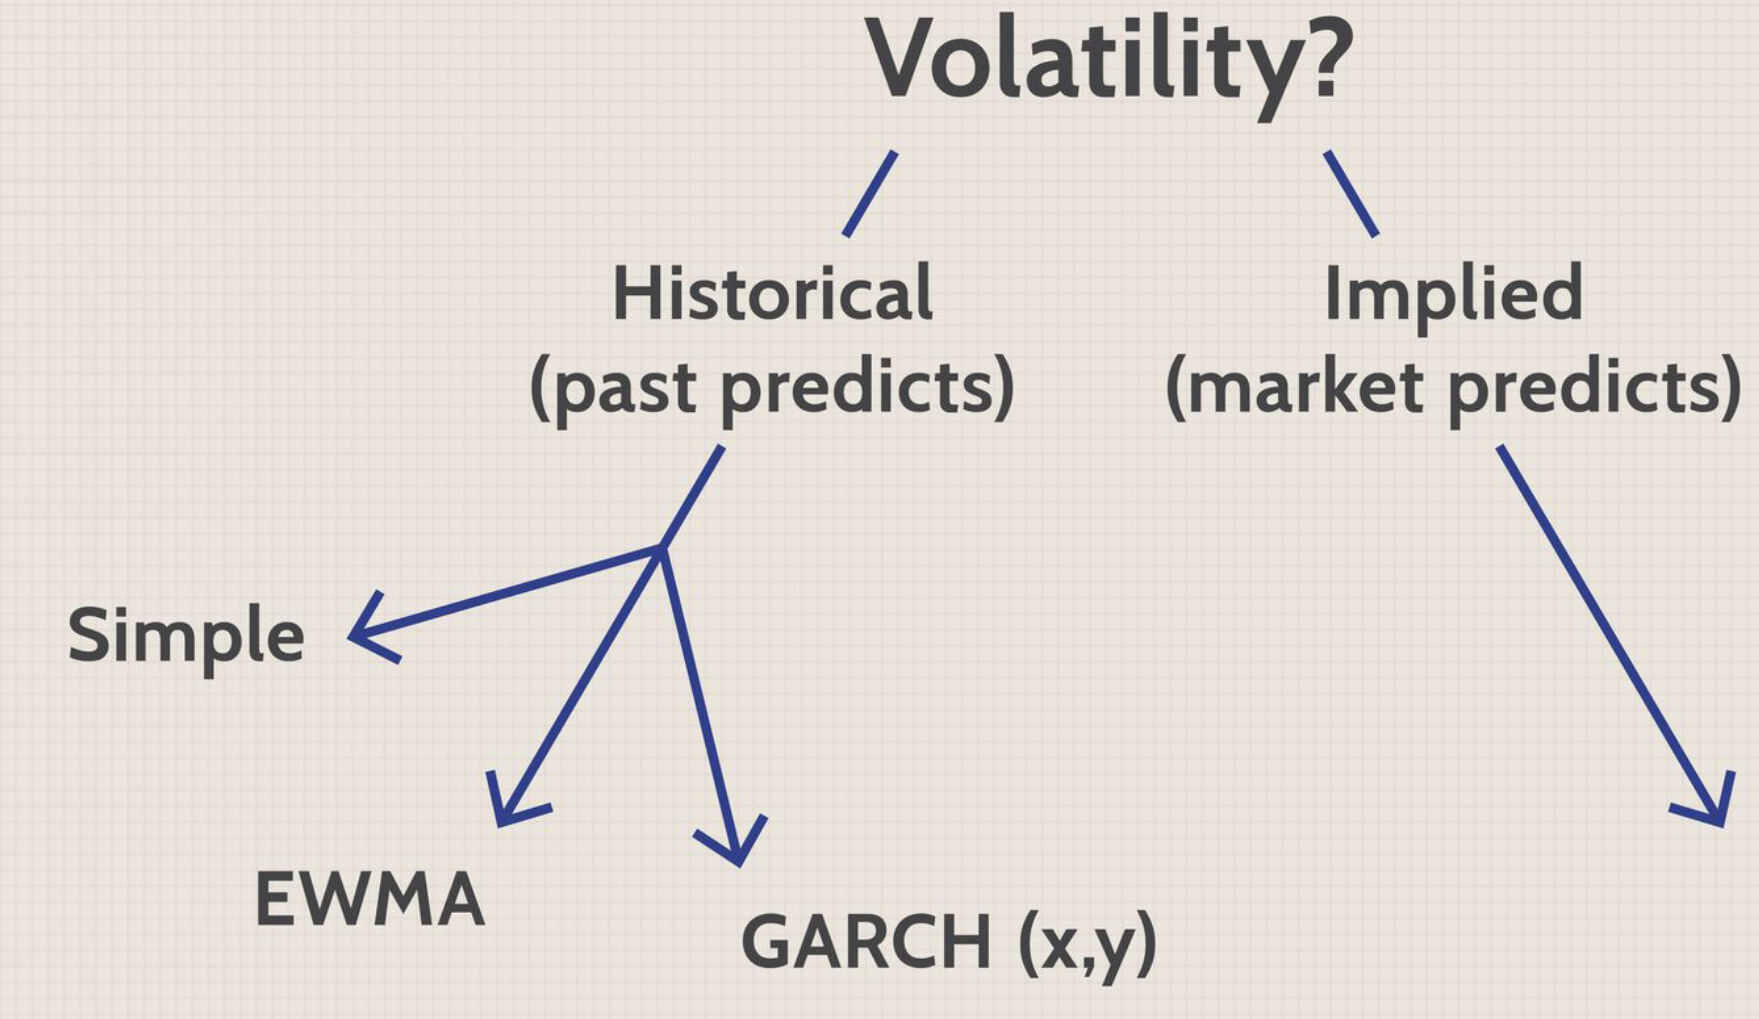
\includegraphics[width=0.75\paperwidth]{static/course_3_img/volatility_decision_tree.PNG}}
%   \hspace*{15pt}\hbox{\scriptsize Credit:\thinspace{\scriptsize\itshape Sabrina Jiang}}          
  
% \end{frame}

% \begin{frame}
%   \frametitle{EWMA Model}
%   \makebox[\linewidth]{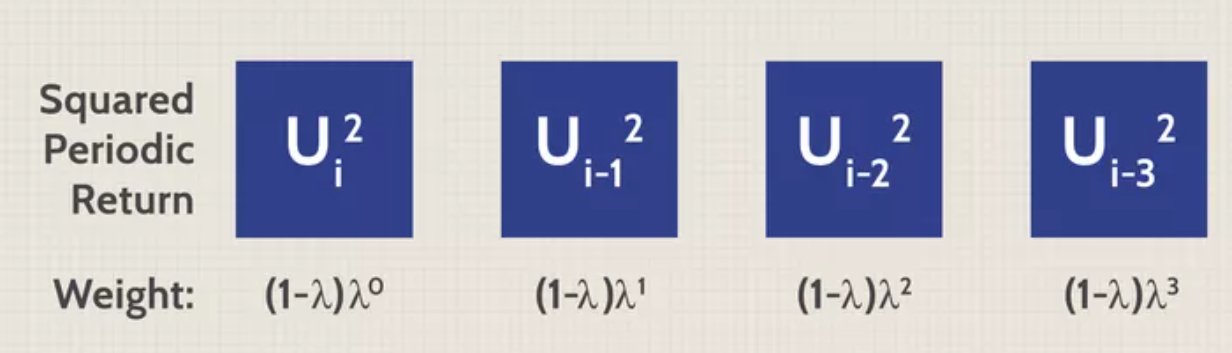
\includegraphics[height=0.35\paperheight]{static/course_3_img/ewma_squared_returns.PNG}}
%   \hspace*{15pt}\hbox{\scriptsize Credit:\thinspace{\scriptsize\itshape Sabrina Jiang}}          

%   \medskip

%   \makebox[\linewidth]{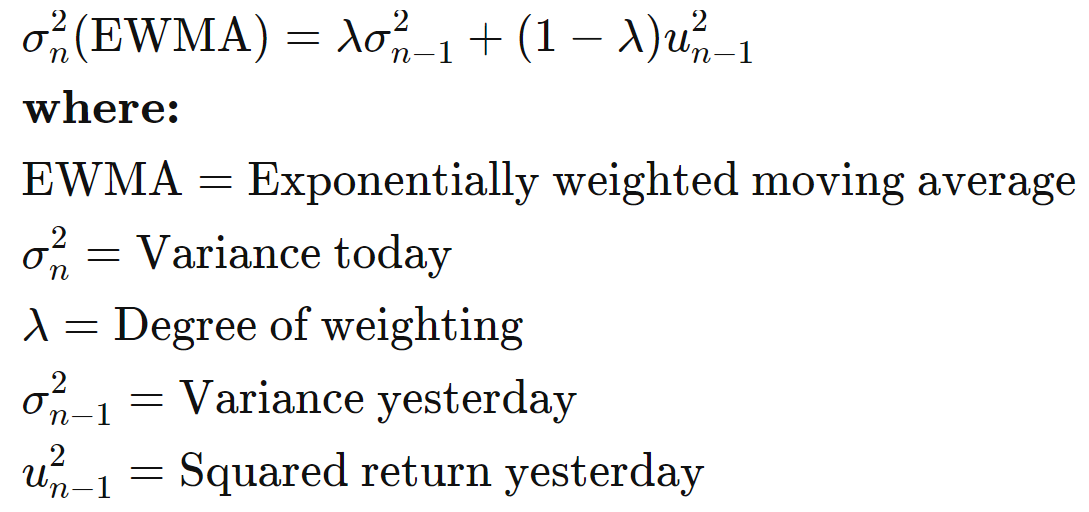
\includegraphics[height=0.35\paperheight]{static/course_3_img/ewma_formula.PNG}}
%   %\hspace*{15pt}\hbox{\scriptsize Credit:\thinspace{\scriptsize\itshape Sabrina Jiang}}          
  
% \end{frame}


% \begin{frame}
%   \frametitle{EWMA Weights}
%   \makebox[\linewidth]{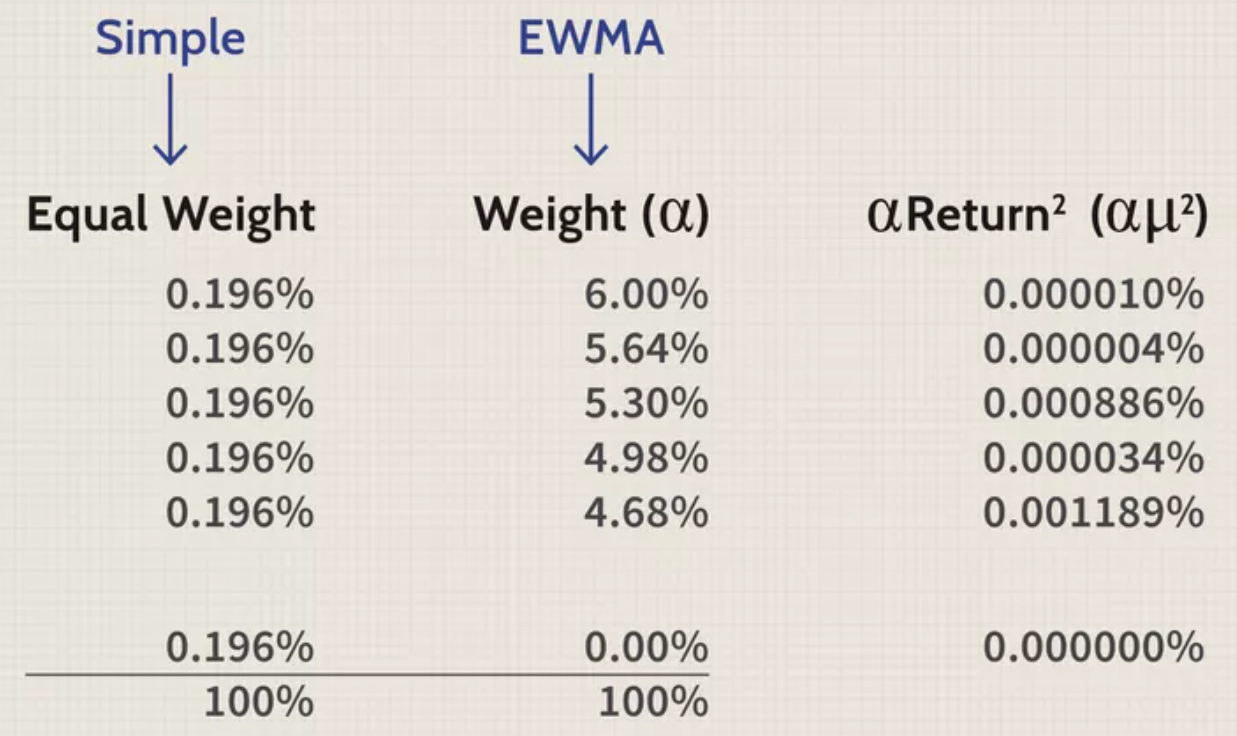
\includegraphics[height=0.65\paperheight]{static/course_3_img/ewma_weights.PNG}}
%   %\hspace*{15pt}\hbox{\scriptsize Credit:\thinspace{\scriptsize\itshape Sabrina Jiang}}            
% \end{frame}
\section{Introduction}
\begin{frame}{Challenges in estimating volatility}
\small
    \begin{itemize}
        \item Daily volatility is unobserved, and can not be derived from the daily returns $R_t$ because there is only one observation in a trading day t
        \item Volatility of price returns is not static, It changes frequently for several reasons
    \end{itemize}
    
\textbf{Why does volatility change?}
     \begin{itemize}
         \item \imfbold{News Announcements}: Macroeconomic and earnings announcement. As new information arrives, uncertainty rises regarding interpreting it and reshuffling portfolios.
         \item \imfbold{State of Uncertainty}: Brexit, Trump election, Covid-19, SVB 
         \item \imfbold{Illiquidity}: Price movement upon taking directional bets on illiquid assets is high 
         \item \imfbold{Volatility Feedback}: Market-Makers behavior, fleeing the order book when volatility increase (when it matters the most)
         \item \imfbold{Leverage}:An price declines, companies become more
leveraged (debt-to-equity ratio up) and riskier
     \end{itemize}
\end{frame}
\begin{frame}{Volatility Estimates}
    \begin{enumerate}
    \item \imfbold{ Realized Volatility}, but on what window ?
        $$ \hat{\sigma} = \sqrt{ \frac{1}{T} \sum_{t=1}^T (r_t - \hat{\mu})}$$
    
    \item \imfbold{Implied volatility} the volatility which when input in an option pricing model (such as Black-Scholes) will return the market price of the option. Example: the CBOE Volatility Index (ticker: VIX).
    \item \imfbold{High Frequency Data Estimators}. The realized volatility is computed as the sum of squared intraday returns (Andersen and Bollerslev, 1998).
\item The \imfbold{Conditional Volatility} issued from dynamic models such as the \textbf{ARCH} and \textbf{GARCH} type models $\Esp_t[\sigma_{t+1}^2]$
 
\end{enumerate}
\end{frame}
\begin{frame}{Volatility Estimates}
    \begin{enumerate}
    \item \imfbold{ Realized Volatility}, but on what window ?
        $$ \hat{\sigma} = \sqrt{ \frac{1}{T} \sum_{t=1}^T (r_t - \hat{\mu})}$$
    
    \item \imfbold{Implied volatility} the volatility which when input in an option pricing model (such as Black-Scholes) will return the market price of the option. Example: the CBOE Volatility Index (ticker: VIX).
    \item \imfbold{High Frequency Data Estimators}. The realized volatility is computed as the sum of squared intraday returns (Andersen and Bollerslev, 1998).
\begin{tcolorbox}[colframe=red, colback=white]
\item The \imfbold{Conditional Volatility} issued from dynamic models such as the \textbf{ARCH} and \textbf{GARCH} type models $\Esp_t[\sigma_{t+1}^2]$
\end{tcolorbox}    
\end{enumerate}
\end{frame}

\begin{frame}{Stylized Facts of Financial Time series}
How ARCH/GARCH models cover the properties of financial time series?
    \begin{enumerate}
        \item The returns are stationary 
        \item Absence of autocorrelations 
        \item Heavy tails 
        \item Asymmetry
        \item Volatility clustering 
        \item Aggregational Gaussianity
        \item ARCH effect 
        \item Leverage effect
    \end{enumerate}
\end{frame}

\section{ARCH Models}
\begin{frame}{ARCH Models}
The ARCH model has been introduced by \imfbold{ Engle (1982)}
\begin{center}
    \textbf{\color{red}ARCH} = \textbf{\color{red}A}uto\textbf{\color{red}R}egressive \textbf{\color{red}C}onditional \textbf{\color{red}H}eteroskedasticity\\
    Robert F. Engle Nobel Prize 2003
\end{center}
\pause
\medskip
\begin{itemize}
    \item The squared return follows an \imfbold{autoregressive model}.
    \item The term \imfbold{ heteroscedasticity} refers to a time-varying variance.
    \item In an ARCH model, it is the \imfbold{conditional variance} (and not the variance itself) that changes with time, in a specific way, depending on the available data.    
\end{itemize}   
\end{frame}

\begin{frame}{ARCH Models}
    \begin{block}{Definition: ARCH(q)}
       The process {$X_t, t\in \Z$} is said to be an ARCH(q) process, if 
       $$X_t = Z_t\sigma_t$$
       where $Z_t$ is a sequence of independent and identically distributed (i.i.d.) random variables with $\Esp(Z_t) = 0$ and $\Var(Z_t) = 1$,
       and $\sigma_t$ is a non-negative process such that
       $$\sigma_t^2 = \alpha_0 + \sum_{i-1}^P {\alpha_{i}X_{t-i}^2}$$
       with $\alpha_0>0,~ \alpha_i \in \R, \quad \forall i<P, \alpha_p\in \R^*$ and $ \sum_{i-1}^P {\alpha_{i}} <1$ 
    \end{block}
\end{frame}

% \begin{frame}{Focus on ARCH(1)}
%     \begin{block}{Definition: ARCH(1)}
%        The process {$X_t, t\in \Z$} is said to be an ARCH(1) process, if 
%        $$X_t = Z_t\sigma_t$$
%        where $Z_t$ is a sequence of independent and identically distributed (i.i.d.) random variables with $\Esp(Z_t) = 0$ and $\Var(Z_t) = 1$,
%        and $\sigma_t$ is a non-negative process such that
%        $$\sigma_t^2 = \alpha_0 +\alpha_1X_{t-1}^2$$
%        with $\alpha_0>0$ and $0 \leq \alpha_1 <1$
%     \end{block}
% \end{frame}

\begin{frame}{Interpretation}
Consider an ARCH(1) process 
\begin{align*}
    X_t & = Z_t\sigma_t\\
    \sigma_t^2 &= \alpha_0 +\alpha_1X_{t-1}^2
\end{align*}
Then we have 
$$ \Var(X_t|\underline{X}_{t-1}) = \Var(Z_t\sigma_t|\underline{X}_{t-1}) = \sigma_t^2\Var(Z_t|\underline{X}_{t-1}) =\sigma_t^2\Var(Z_t) = \sigma_t^2$$
       \begin{itemize}
           \item Given the past information $\underline{X}_{t-1}$, the conditional variance $\sigma_t^2 = \alpha_0 +\alpha_1X_{t-1}^2$ is \imfbold{ deterministic}, since $x_{t-1}$ is a constant
           \item The process {$Z_t, t\in \Z$} is an i.id noise, so $\Var(Z_t|\underline{X}_{t-1}) = \Var(Z_t)$ i.e. there is no memory in $Z_t$
           \item The normalization $\Var(Z_t)=1$ is not a restriction: the scaling implied by any other variance would be absorbed by the parameters $\alpha_0$ and $\alpha_1$
       \end{itemize}
\end{frame}

\begin{frame}{Conditional Variance}
    \begin{block}{Definition}
        The process $\sigma_t^2$ corresponds to the \textbf{conditional variance} of $X_t$
        $$\Var(X_t|\F_{t-1}) \equiv \Var(X_t|\underline{X}_{t-1}) = \sigma_t^2 $$
        where $\F_{t-1} \equiv \underline{X}_{t-1} = \{X_{t-1}, X_{t-2}, ... \}$ is the information set available at time $t-1$
    \end{block}
    \vspace{2pt}
    Some authors denote the conditional variance by $h_t$, with 
    \begin{align*}
        X_t &= Z_t\sqrt{h_t}\\
        h_t & = \alpha_0 +\alpha_1X_{t-1}^2
    \end{align*}  
\end{frame}
\begin{frame}{Key properties of ARCH models}
If {$X_t,~t \in \Z$} has an ARCH(1) representation with Gaussian innovations, then
\begin{enumerate}
    \item $X_t^2$ has an AR(1) representation
    \item $X_t$ is a martingale difference
    \item $X_t$ is a stationary process under some conditions on the parameters
    \item $X_t$ is (unconditionally) Homoscedastic
    \item $X_t$ is conditionally Heteroscedastic
    \item The (marginal) distribution of $X_t$ is leptokurtic
    \item The conditional distribution of $X_t$ is normal    
\end{enumerate}
\end{frame}

\begin{frame}{Property 1:}
\begin{block}{Definition}
    If $\{ X_t, t\in\Z\}$ has an ARCH(1) representation, with
    \begin{align*}
        X_t & = Z_t\sigma_t\\
        \sigma_t^2 &= \alpha_0 +\alpha_1X_{t-1}^2
    \end{align*}
If $\{ X_t^2, t\in\Z\}$ has an AR(1) representation, with
$$X_t^2 = \alpha_0 +\alpha_1X_{t-1}^2 + \nu_t$$
where $\nu_t$ is an innovation process 
$$\Esp[\nu_t|\underline{X}_{t-1}] =0$$
\end{block}    
\imfbold{Consequences}
$X_t^2$ and $X_{t-k}^2$ are correlated $\Rightarrow$ \textbf{\color{red} ARCH effect}
$$\rho_k = \Corr(X_t^2, X_{t-k}^2) \neq 0$$
especially for small values of k
\end{frame}

\begin{frame}{ARCH Effect}
\centering
    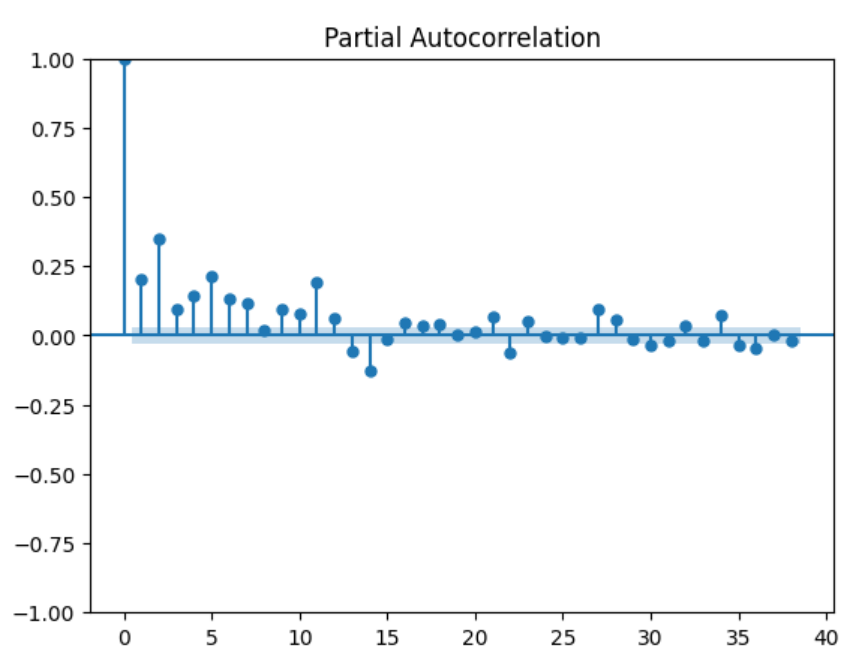
\includegraphics[width=.8\textwidth]{static/course_3_img/PACF_squared_ret.png}
\end{frame}

\begin{frame}{Property 2:}
    \begin{block}{Definition}
        if $\{ X_t, t\in \Z\}$ is an ARCH(1) process, then it is a martingale difference
        $$\Esp[X_t|\F_{t-1}] \equiv \Esp[X_t|\underline{X}_{t-1}] =0 $$
    \end{block}
    \imfbold{Consequences}
    \begin{itemize}
        \item \textbf{The very best} (linear or nonlinear) \textbf{predictor of $X_t$} based on the available information at time $t-1$  \textbf{is} simply the trivial predictor, namely \textbf{the series mean, 0.}
        \item This property implies that $\Cov(X_t,X_{t-k}) =0\quad \forall k \neq 0$, i.e that the process $X_t$ has \textbf{no memory}
        \item In terms of point forecasting of the series itself, then, the ARCH models offer no advantages over the linear ARMA models.
    \end{itemize}
\end{frame}

\begin{frame}{}
\begin{table}[]
    \centering
    \small
    \begin{tabularx}{\linewidth}{*{2}{>{\centering \arraybackslash}X}>{\centering\arraybackslash}p{4.3cm}}
        \imfbold{Innovation} &  \imfbold{ARCH model} & \imfbold{Output}\\
        $Z_t$ i.i.d noise    & $X_t = Z_t\sigma_t$ & $X_t$ is martingale difference \\
        \textbf{No correlation} & $\sigma_t^2 = \alpha_0 +\alpha_1X_{t-1}^2$ & \textbf{No correlation}\\
        between $Z_t$ and $Z_{t-k}$ &                                        & between $X_t$ and $X_{t-k}$\\
                                    &                                        & but $\Cov(X_t^2,X_{t-k}^2) \neq 0$ \\
    \end{tabularx}
\end{table}    
    \begin{block}{ARCH effect}
        The daily squared returns often exhibit significant correlations. These autocorrelations are often referred to as an ARCH effect.
    \end{block}
    \begin{block}{Absence of autocorrelation}
        The \textbf{autocorrelation}  of asset returns $R_t$ are often insignificant, except for very small intraday time scales ($\approx$ 20 minutes) for which microstructure effects come into play.
    \end{block}
\end{frame}

\begin{frame}{Property 3:}
    \begin{block}{Definition}
        if $\{ X_t, t\in \Z\}$ is an ARCH(1) process, then its two first unconditional moments are finite and constant
        $$\Esp[X_t] = 0,\quad\quad \Var(X_t) =\frac{\alpha_0}{1-\alpha_1}, \quad\quad \Cov(X_t, X_{t-k}) =0~ \forall k \neq 0 $$
        with $\alpha_0>0$ and $0 \leq \alpha_1<1$
    \end{block}    
\end{frame}

\begin{frame}{Consequences}
\centering
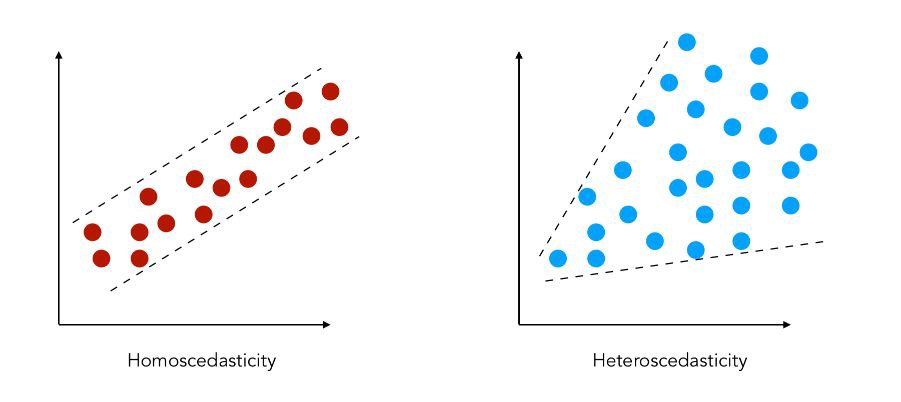
\includegraphics[width=0.8\textwidth]{static/course_3_img/homo_hsk.jpeg}

  \begin{itemize}
        \item An ARCH(1) process is unconditionally \textbf{\color{red} homoscedastic}
        \textbf{Unconditional Variance} $\Var(X_t) =\frac{\alpha_0}{1-\alpha_1}= cst \quad \forall t$
        \item An ARCH(1) process is conditionally \textbf{\color{red} heteroscedastic}
        \textbf{Conditional Variance} $\Var(X_t|\F_{t-1}) =\sigma_t^2 = \alpha_0 + \alpha_1 X_{t-1}^2$ varies with $\F_{t-1}$
        \item An ARCH(1) process is (weakly) \textbf{\color{red}stationary}
\end{itemize}
\end{frame}
\begin{frame}{Consequences}
\centering
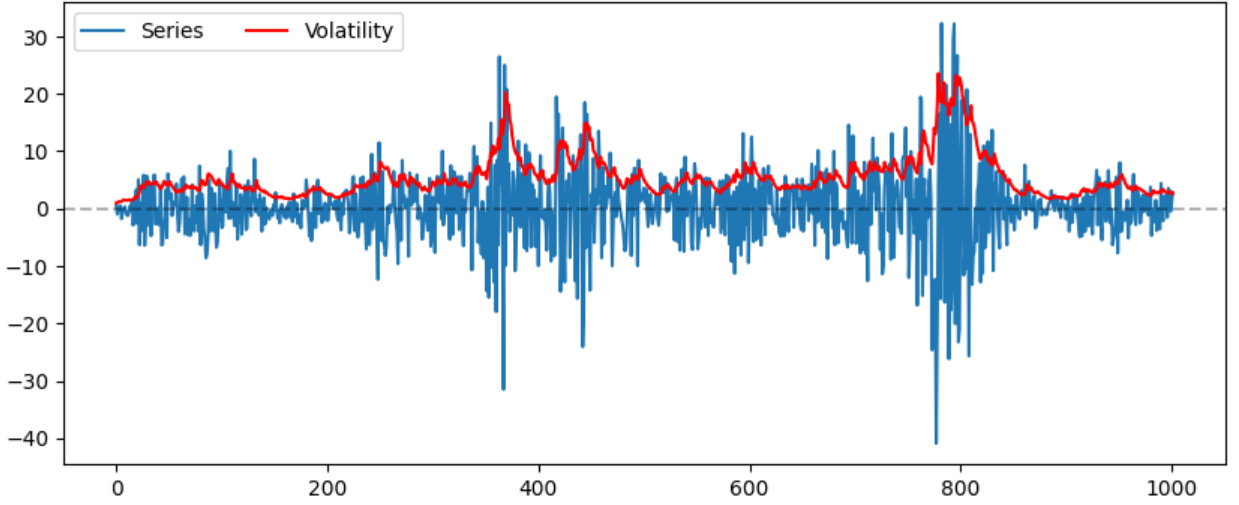
\includegraphics[width=.9\textwidth]{static/course_3_img/simulated_garch22.png}    
\end{frame}

\begin{frame}{Property 4:}
\small
    \begin{block}{Definition}
        if $\{ X_t, t\in \Z\}$ is an ARCH(1) process with Gaussian innovations $Z_t \overset{\mathrm{i.i.d}}{\sim} \N(0,1)$, then, its unconditional and conditional Kurtosis coefficients are equal to
        $$\Kurt(X_t|\underline{X}_{t-1}) = \frac{\Esp(X_t^4|\underline{X}_{t-1})}{{\Var(X_t|\underline{X}_{t-1})}^2} =3 $$
        $$\Kurt(X_t) = \frac{\Esp(X_t^4}{\Var(X_t)^2} = 3 \left( \frac{1-\alpha_1^2}{1-3\alpha_1^2} \right) > 3 \quad if ~\alpha_1<\sqrt{\frac{1}{3}}$$
    \end{block}
    \imfbold{Consequences}
    \begin{itemize}
        \item The return distribution often exhibits \textbf{\color{red}heavier tails} than those of a normal distribution.
        \item Even if the innovation $Z_t$ has a normal distribution, the \textbf{\color{red}marginal distribution} of $X_t$ is not Gaussian
        \item If the innovation $Z_t$ has a normal distribution, the \textbf{\color{red}conditional distribution} of $X_t$ is Gaussian. $X_t|\underline{X}_{t-1} \sim \N(0, \sigma_t^2)$
    \end{itemize}
\end{frame}

\begin{frame}{ARCH models Properties Summary}
 if {$X_t, ~t\in \Z$} is an \textbf{ARCH(1)} process with \textbf{Gaussian innovation}, then
 \small
    \begin{table}
        \centering
        \begin{tabularx}{\linewidth}{m{0.3cm}>{\raggedright\arraybackslash}m{3.7cm} >{\raggedright\arraybackslash}m{7.3cm}}
        \toprule
           & \textbf{Propertry} & \textbf{Consequences / Interpretation}  \\
        \midrule
        \textbf{P1} & $X_t^2$ is an AR(1) process                        & ARCH effect: $\Cov(X_t^2, X_{t-k}^2) \neq 0$ for "small" k\\
        \\
        \textbf{P2} & $X_t$ is a martingale difference                   & $\Esp[X-t|X_{t-1}]=0$ and $\Cov(X_t, X_{t-k}) =0 \quad \forall k\neq 0$ \\
        \\
           & $\Esp[X_t] =0$, & $\{X_t\}$ is stationary,\\ 
        \textbf{P3} &$\Var[X_t] =\frac{\alpha_0}{1-\alpha_1}$, & unconditionally homoscedastic,\\ 
           & $\Var[X_t|X_{t-1}] = \sigma_t^2$  & and conditionally heteroscedastic\\
        \\
                    & $\Kurt[X_t]>3$,&  The ARCH model generates leptokurtosis,\\
        \textbf{P4} &$\Kurt[X_t|X_{t-1}]=3$ & The \textbf{marginal distribution} of $X_t$ is not Gaussian,\\
                    && The \textbf{conditional distribution} of $X_t$ is Gaussian\\
        \bottomrule
        \end{tabularx}
        \label{tab:my_label}
    \end{table}
    
\end{frame}

\begin{frame}{ARCH(1) models fits most of the stylized facts of financial series}
    The properties of the ARCH(1) allow to capture most of the stylized facts of financial data (cf. Chapter 1) 
    \begin{enumerate}
        \item \imfbold{The returns are stationary} $\Rightarrow {X_t}$ is stationary
        \item \imfbold{Absence of autocorrelations} $\Rightarrow {X_t}$ is a martingale difference
        \item \imfbold{Heavy tails} $\Rightarrow {\Kurt(X_t)}$ may be larger than 3 given the value of $\alpha_1$
        \item \textbf{\color{red}Asymmetry}
        \item \imfbold{Volatility clustering} $\Rightarrow {\Cov(X_t^2, X_{t-k}^2) \neq 0}$
        \item \imfbold{Aggregational Gaussianity} $\Rightarrow$ The marginal distribution of $X_t$ is not normal
        \item \imfbold{ARCH effect} $\Rightarrow {X_t}^2$ has an AR(1) representation and ${\Cov(X_t^2, X_{t-k}^2) \neq 0}$
        \item \textbf{\color{red}Leverage effect}
    \end{enumerate}
\end{frame}

\begin{frame}{Building an ARCH model}
    Denote by $R_t$ the \imfbold{daily return} of an asset or a portfolio at time t.
    
    $$R_t = \underset{\substack{\mathrm{conditional} \\ \mathrm{mean~model}}} {\underbrace{\mu_t}} + \underset{\substack{\mathrm{innovation} \\ \mathrm{(martingale~diff)} }}{\underbrace{\epsilon_t}} $$
    $$\epsilon_t = Z_t\sigma_t$$
    $$\sigma_t^2 = \underset{\substack{\mathrm{conditional} \\ \mathrm{variance~model}}} {\underbrace{\alpha_0 + \sum_{i-1}^P {\alpha_{i}X_{t-i}^2} }}$$
    follows the structure of a \textbf{(conditional) volatility model}
    $$\mu_t \equiv \Esp(R_t|\F_{t-1}) =  \mu_t(\underline{R}_{t-1};\theta) $$
    $$\sigma_t^2 \equiv \Var(R_t|\F_{t-1}) = \sigma_t^2(\underline{R}_{t-1};\theta)$$
    where $\theta$ denotes the \textbf{set of parameters} for the conditional mean and variance and $\mu_t$ is typically an \textbf{ARMA}-type model .

\end{frame}

\begin{frame}{Example}
    \begin{exampleblock}{Example ARMA(1,1)-ARCH(1)}
    \small
    The process $\{R_t, ~t\in\Z\}$ has an \textbf{ARMA(1,1)-ARCH(1)} representation if
        $$R_t = \phi_0 + \phi_1 R_{t-1}+ \theta_1\epsilon_{t-1} + \epsilon_t $$
        $$\epsilon_t = Z_t\sigma_t$$
        $$\sigma_t^2 = \alpha_0 + \alpha_1\epsilon_{t-1}^2$$
        where $Z_t$ is a sequence of i.i.d. variables with $\Esp(Z_t)=0$ and $\Var(Z_t)=1$. 
        
        We have
        $$\mu_t = \Esp(R_t|\F_{t-1}) =  \phi_0 + \phi_1 R_{t-1}$$
        $$\sigma_t^2 =\Var(R_t|\F_{t-1}) = \alpha_0 + \alpha_1\epsilon_{t-1}^2$$
        and $\theta = (\phi_0, \phi_1, \theta_1, \alpha_0, \alpha_1)' $ is the vector of parameters to estimate
    \end{exampleblock}
\end{frame}

% \begin{frame}{Estimation methods}
%     Estimation: The parameters $\theta$ are estimated by
%     \begin{enumerate}
%         \item Maximum Likelihood (ML) when one puts a distributional assumption on the innovations term $Z_t$
%         \item Quasi Maximum Likelihood (QML) when the distribution of $Z_t$ is unknown. The QML only assumes that the true (unknown) distribution of $Z_t$ belongs to a given family (typically the exponential family).
%         \item In most statistical software, the model parameters are estimated by ML and the normality assumption is considered by default.
%         $$Z_t \overset{\mathrm{i.i.d}}{\sim} \N(0,1) $$
%     \end{enumerate}
% \end{frame}

\begin{frame}{Model Checking}
    \begin{itemize}
        \item For an ARCH model, the \textbf{standardized innovations} $Z_t = \frac{\epsilon_t}{\sigma_t}$
        are i.i.d. random variates (following for example a standard normal or Student-t distribution).
        \item Therefore, one can check the adequacy of a fitted ARCH model by examining the series of \textbf{standardized residuals}
        $$\hat{Z_t} = \frac{\hat{\epsilon_t}}{\hat{\sigma_t}}$$
    \end{itemize}
    
    \begin{enumerate}
        
        \item The skewness, kurtosis, and QQ-plot of $\hat{z_t}$ can be used to check the validity of the distribution assumption on $Z_t$.

        \item Kolmogorov-Smirnov test on $\hat{z}_t$
    \end{enumerate}
\end{frame}

\begin{frame}{Forecasting}
\small
We have to distinguish:
\begin{itemize}
    \item The forecasts on the series $R_t$ itself (typically the returns).
    \item The forecasts on the volatility (or the variance) of $R_t$.
\end{itemize}
\begin{alertblock}{Forecasting of the series $R_t$}
    The best linear forecast of $R_t$ given the information set $\F_{t-1}$ will be no different \textbf{with or without} an ARCH error %because the process $\epsilon_t$ is a martingale difference
\end{alertblock}
\end{frame}
\begin{frame}{Weaknesses of ARCH Models}

\begin{enumerate}
    \item It requires a \textbf{large order (q)} to calibrate the model on financial data 
    \item The model \textbf{assumes positive and negative shocks have the same effects on volatility} because it depends on the square of the previous shocks. 
    
    \item  The ARCH model provides \textbf{no insight into understanding the source of volatility}. It only provides a \emph{mechanical way} to describe the behavior of the conditional variance.
    
    \item The ARCH model is rather restrictive. For instance, the fourth moment $\Esp(X_t^4)$ exists only if $\alpha_1^2< \frac{1}{3}$
\end{enumerate}   
\end{frame}


\section{GARCH Models}
\begin{frame}{GARCH Models}
Due to the large persistence in volatility, ARCH models often require a large p to fit the data. A more parsimonious specification is provided by \imfbold{GARCH} models.
\medskip
\begin{center}
    \textbf{\color{red}GARCH} = \textbf{\color{red}G}eneralized \textbf{\color{red}A}uto\textbf{\color{red}R}egressive \textbf{\color{red}C}onditional \textbf{\color{red}H}eteroskedasticity\\
    Bollerslev, T. (1986)
\end{center}
\end{frame}


\begin{frame}
\begin{block}{Definition: GARCH Model}
  The stochastic process $\{ \epsilon_t, \ t \in \mathbb{Z} \}$ is said to be a \textbf{GARCH}(p,q) process if:
  $$\epsilon_t = Z_t \sigma_t$$
  where $Z_t$ is a sequence of i.i.d variables with $\mathbb{E}(Z_t) = 0$ and $\mathbb{V}(Z_t) = 1$, and $\sigma_t$ is a non-negative process such that:
    $$\sigma^2_t = \omega + \sum^p_{i=1} \alpha_i \epsilon^2_{t-i} + \sum^p_{i=1} \beta_i \sigma^2_{t-i}$$
  with $\omega >0$, $\forall \ i, (\alpha_i, \beta_i) \ \in \ \mathbb{R}^{+,2}$ and $\sum^p_{i=1} \alpha_i + \sum^p_{i=1} \beta_i <1$  
\end{block}
\end{frame}


\begin{frame}
  \frametitle{GARCH: Intuition}
  \begin{wideitemize}
  \item The conditional variance of a GARCH(p, q) depends on:
    \begin{itemize}
    \item The first p lag of the $\epsilon_t^2$ (e.g. the squared error terms)
    \item The first $q$ lag of the conditional variance $\sigma^2$
    \end{itemize}
 \begin{equation*}
    \sigma^2_t = \omega + \underbrace{\sum^p_{i=1} \alpha_i \epsilon^2_{t-i}}_{\text{ARCH Components}} + \underbrace{\sum^p_{i=1} \beta_i \sigma^2_{t-i}}_{\text{GARCH components}}
  \end{equation*}   
   
  \item The parameters $\alpha_i$ are often called the \textbf{ARCH parameters}
  \item The parameters $\beta_i$ are often called the \textbf{GARCH parameters}
\end{wideitemize}
  
\end{frame}

\begin{frame}
  \frametitle{GARCH(1, 1)}

  \begin{alertblock}{Tip: Does anything beat GARCH(1,1)}
GARCH(1,1) specifications are generally sufficient to capture the dynamics of the conditional variance
  \end{alertblock}

  \medskip
  
\begin{block}{Special Case: GARCH(1, 1)}

  The process $\{ \epsilon_t, \ t \in \mathbb{Z} \}$ is said to be a \textbf{GARCH}(1,1) if:
  $$\epsilon_t = Z_t \sigma_t$$
  where $Z_t$ is a sequence of i.i.d variables with $\mathbb{E}(Z_t) = 0$ and $\mathbb{V}(Z_t) = 1$, and $\sigma_t$ is a non-negative process such that:
  $$\sigma^2_t = \omega + \alpha \epsilon^2_{t-1} + \beta \sigma^2_{t-1}$$
  with $\omega >0$, $\alpha \geq 0, \beta \geq 0$ and $\alpha + \beta <1$  
\end{block}
\end{frame}


\begin{frame}
  \frametitle{Conditional Variance Persistences}
  \small
  \begin{itemize}
  \item The conditional variance $\sigma_t^2 = \omega + \alpha \epsilon^2_{t-1} + \beta \sigma^2_{t-1}$ depends on two effects:
    \begin{itemize}
    \item An \textbf{intrinsic persistence} effect through the first lag of the conditional variance
    \item An \textbf{extrinsic persistence} effect
    \end{itemize}    
  \item Following a positive (or negative) shock at time \emph{t-1}, the conditional variance at time \emph{t} increases (impact effect) and thus it has an impact on $\epsilon_t = Z_t \sigma_t$
        $$\text{shock} \ z_{t-1} \ > \ 0 \Rightarrow \ \epsilon_{t-1} \ \uparrow \ \Rightarrow \ \sigma_t \ \uparrow \ \dots$$  
  \item Starting from the next period (at time $t$), the effect of the shock at $t-1$ on the conditional variance at $t+1$ passes through the conditional variance at time $t$ (intrinsic persistence)
    $$... \ \Rightarrow \ \sigma_t \ \uparrow \ \Rightarrow \ \sigma^2_{t+1} \ \uparrow $$    
    \item The overall effect of a shock can be decomposed into a \imfbold{contemporaneous effect}, which depends on $\alpha$ and a \imfbold{persistence effect} that depends on $\beta$    
  \end{itemize}
\end{frame}

\begin{frame}{Remarks}

   It is often the case that:
    \begin{wideenumerate}
      \item The sum of the estimates of $\alpha$ and $\beta$ are generally close, but below, 1
      \item The estimate of $\beta$ is generally greater than the one of $\alpha$
      \item The estimate of $\beta$ is generally larger than 0.90 for daily returns and the estimate of $\alpha$ is below 0.1
  \end{wideenumerate}
  Be careful: it is not a general rule, just an observation.
\end{frame}
\begin{frame}{GARCH Properties}
\small
GARCH process properties are similar to those of an ARCH process.
\begin{enumerate}
    \item ARCH properties
    \item $\epsilon_t^2$ has an ARMA representation
\end{enumerate}
\begin{block}{ARMA representation}
  If $\{ \epsilon_t, \ t \in \mathbb{Z} \}$ has a \textbf{GARCH}(p,q) representation with:
  $$\epsilon_t = Z_t \sigma_t$$
  $$\sigma^2_t = \omega + \sum^p_{i=1} \alpha_i \epsilon^2_{t-i} + \sum^p_{i=1} \beta_i \sigma^2_{t-i}$$
  the $\{ \epsilon_t^2, \ t \in \mathbb{Z} \}$ has a \textbf{ARMA}(max(p,q), q) representation with: 
  $$\epsilon^2_t = \omega + \sum^p_{i=1} (\alpha_i + \beta_i) \epsilon^2_{t-i} + \nu_t - \sum^p_{i=1} \beta_i \nu_{t-i}$$
  with $\nu = \epsilon^2_t - \sigma^2_t$ is an innovation process, i.e $\Esp(\nu_t|\F_{t-1})$
\end{block}    
\end{frame}

\begin{frame}{Distributions}
The most often used distributions for $Z_t$ are:
\centering
    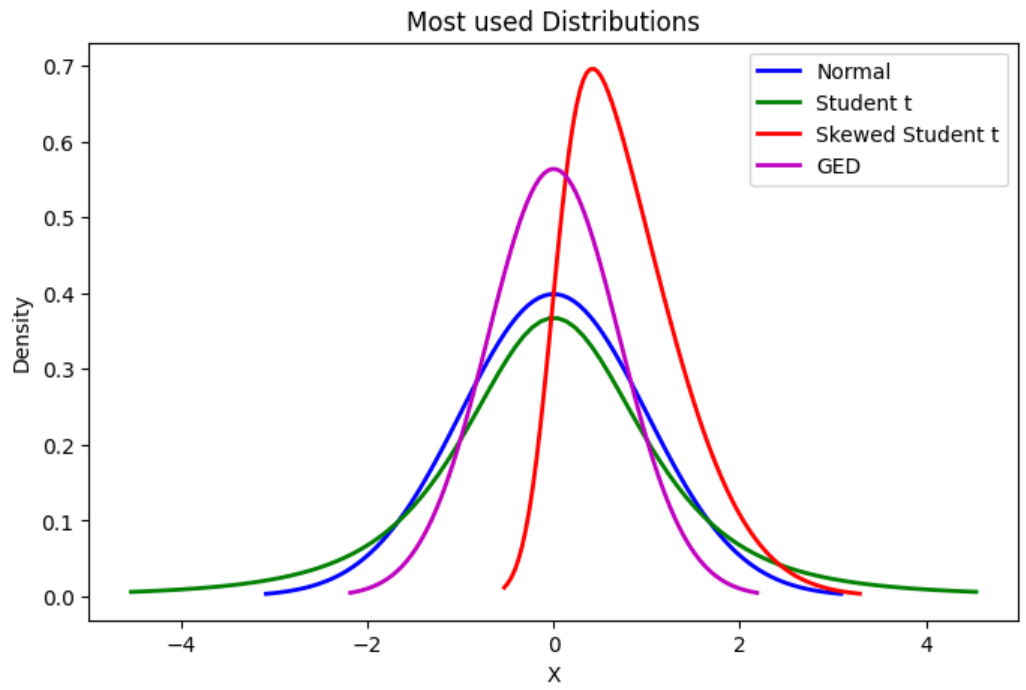
\includegraphics[width=.9\textwidth]{static/course_3_img/common_distrib.png}
\end{frame}
\begin{frame}{Distributions}
The most often used distributions for $Z_t$ are:
        \begin{enumerate}
            \item The \imfbold{normal distribution}, $Z_t \overset{\mathrm{i.i.d}}{\sim} \N(0,1)$. IMPORTANT: the normality assumption on $Z_t$ does not imply that the return $R_t$ has a normal (marginal) distribution.
            \item The \imfbold{Student t-distribution}, $Z_t \overset{\mathrm{i.i.d}}{\sim} t(\nu)$ , which is symmetric and leptokurtic (if $\nu$ is "small").
            \item The \imfbold{skewed Student t-distribution}, $Z_t \overset{\mathrm{i.i.d}}{\sim} Skewed~t(\delta,\nu)$, which is asymmetric (if $\delta \neq 1$) and leptokurtic (if $\nu$ is "small").
            \item The \imfbold{Generalized Error Distribution (GED)}, $Z_t \overset{\mathrm{i.i.d}}{\sim} GED(\nu)$, which is symmetric and leptokurtic (if $\nu$ < 2).
        \end{enumerate}

\end{frame}

\begin{frame}{Remark}
\small
    Why consider non-Gaussian distributions for the innovation $Z_t$?
    \begin{enumerate}
        \item The use of a \imfbold{leptokurtic distribution} for $Z_t$ allows to increase the kurtosis of $R_t$.
        \begin{align*}
          \text{Kurtosis of a GARCH process}  &= \text{kurtosis generated by the model} \\
                                              &+ \text{ kurtosis of the innovation } Z_t  
        \end{align*}
        The kurtosis generated by the model dynamic is generally not sufficient to reproduce the level of kurtosis observed in the financial returns.

        \item The use of a \imfbold{skewed distribution} for $Z_t$ allows to reproduce the skewness observed in the distribution of the financial returns.
        $$ \text{Skewed distribution for }Z_t \Rightarrow \text{Skewed distribution for }R_t$$
    \end{enumerate}
\end{frame}

\section{GARCH Extensions}
\begin{frame}{Asymmetric GARCH models}
\begin{itemize}
    \item The GARCH model assumes that positive and negative shocks have the same effects on volatility because it depends on the square of the previous shocks.
    \item In practice, the return of a financial asset responds differently to positive and negative shocks.
    \item The GARCH model does not allow to capture the \imfbold{leverage effect}. 
\end{itemize}
\end{frame}

\begin{frame}{Asymmetric GARCH models}
    \begin{block}{Stylized Fact 8: Leverage Effect}
        Asset returns are negatively correlated with the changes in their volatilities: this negative correlation is called the leverage effect
    \end{block}
    \medskip
    \begin{itemize}
        \item As asset prices decline, companies become more leveraged (debt-to-equity ratios increase) and riskier, and hence their stock prices become more volatile.
        \item On the other hand, when stock prices become more volatile, investors demand high returns, and hence stock prices go down.
        \item Many asymmetric GARCH models have been proposed: \textbf{GJR-GARCH, TGARCH, EGARCH}, APARCH, VSGARCH, QGARCH, LSTGARCH, ANSTGARCH, etc.
    \end{itemize}
\end{frame}

\begin{frame}{GJR-GARCH}
    One of the most often used asymmetric models is the \imfbold{GJR-GARCH} model, where "GJR" stands for Glosten, Jagannathan, and Runkle (1993).
    \begin{block}{Definition}
        The process $\{\epsilon_t, t \in \Z\}$ is to be a \textbf{GJR-GARCH(1,1)} process, if
        $$\epsilon_t = Z_t\sigma_t$$
        where $Z_t$ is i.i.d with $\Esp(Z_t) = 0$ and $\Var(Z_t)=1$, and 
        
        $$\sigma_t^2 = w+\alpha\epsilon_{t-1}^2 + \gamma \mathbb{I}_{(\epsilon_{t-1}>0)}\epsilon_{t-1}^2 + \beta \sigma_{t-1}^2$$
        with $w>0, \quad \alpha>0, \quad \beta>0, \quad \gamma \in \R$ and where  $\mathbb{I}_{(.)}$ is the indicator function that takes a value 1 if the condition is true and 0 otherwise.
    \end{block}
\end{frame}

\begin{frame}{GJR-GARCH Interpretation}
    \begin{itemize}
        \item The term $\epsilon_t$ can be interpreted as a shock (surprise) on the return, since
        $$\epsilon_t = R_t - \mu_t = R_t - \Esp(R_t|\F_{t-1})$$
        \item In a \textbf{GJR-GARCH} model, the influence of the past return shock $\epsilon_t$ on the current conditional variance $\sigma_t^2$ depends on its sign
        $$\sigma_t^2 = w+\alpha\epsilon_{t-1}^2 + \gamma \mathbb{I}_{(\epsilon_{t-1}>0)}\epsilon_{t-1}^2 + \beta \sigma_{t-1}^2$$
        $$\frac{\partial\sigma_t^2}{\partial\epsilon_{t-1}^2} = \left\{
        \begin{matrix}
                         \alpha + \gamma & if \epsilon_{t-1} <0\\ 
                         \alpha & otherwise
        \end{matrix}
        \right\}.$$
        \item A \imfbold{leverage effect} implies that $\gamma > 0$, i.e. the increase in volatility caused by a negative return is larger than the appreciation due a positive return of the same magnitude.
    \end{itemize}
\end{frame}

\begin{frame}{TGARCH model}
\begin{itemize}
    \item The TGARCH, where "T" stands for \imfbold{Threshold}, is an asymmetric GARCH model designed to capture the leverage effect.
    \item The TGARCH is similar to the GJR model, different only because of the use of the \imfbold{conditional volatility}, instead of the variance, in the specification.
    \item The TGARCH has been introduced by Zakoian (1994).
\end{itemize} 
\end{frame}

\begin{frame}{TGARCH}

    \begin{block}{Definition}
        The process $\{\epsilon_t, t \in \Z\}$ is to be a \textbf{TGARCH(1,1)} process, if
        $$\epsilon_t = Z_t\sigma_t$$
        where $Z_t$ is i.i.d with $\Esp(Z_t) = 0$ and $\Var(Z_t)=1$, and 
        $$\sqrt{\sigma_t^2} = w+\alpha_{+}\epsilon_{t-1}\mathbb{I}_{(\epsilon_{t-1}>0)}+\alpha_{-}\epsilon_{t-1}\mathbb{I}_{(\epsilon_{t-1}<0)} + \beta\sqrt{\sigma_{t-1}^2}$$
        with $(w,\alpha_{+},\alpha_{-}, \beta) \in \R^4$ and $\mathbb{I}_{(.)}$ is the indicator function
    \end{block}
\end{frame}
\begin{frame}{TARCH Interpretation}
    \begin{itemize}
        \item One advantage of the TGARCH is that it does not require any \imfbold{positivity constraints} on the parameters, since we have $\forall (w,\alpha_{+},\alpha_{-}, \beta) \in \R^4$
        $$\sigma_t = \left( w+\alpha_{+}\epsilon_{t-1}\mathbb{I}_{(\epsilon_{t-1}>0)}+\alpha_{-}\epsilon_{t-1}\mathbb{I}_{(\epsilon_{t-1}<0)} + \beta\sqrt{\sigma_{t-1}^2} \right) \geq 0$$
        \item The \imfbold{TGARCH} allows to capture an \imfbold{asymmetry} between positive and negative shocks, as 
        $$\frac{\partial\sigma_t}{\partial\epsilon_{t-1}} = \left\{
        \begin{matrix}
                         \alpha_{-} & if \epsilon_{t-1} <0\\ 
                         \alpha_{+} & otherwise
        \end{matrix}
        \right\}.$$
        \item The \imfbold{leverage effect} implies that $|\alpha_{-} > \alpha_{+}|$, i.e. the increase in volatility caused by a negative return is larger than the appreciation due to a positive return of the same magnitude
    \end{itemize}
\end{frame}

\begin{frame}{EGARCH model}
    \begin{itemize}
        \item "E" stands for \imfbold{Exponential}. The EGARCH has been introduced by Nelson (1991).
        \item It was designed to capture both (1) the asymmetric effects and (2) the effects of "big" shocks.     
    \end{itemize}
    \begin{block}{Definition}
        The process $\{\epsilon_t, t \in \Z\}$ is to be a \textbf{EGARCH(1,1)} process, if
        $$\epsilon_t = Z_t\sigma_t$$
        $$ln(\sigma_t^2) =w + \alpha~ Z_{t-1} + \gamma\left(|Z_{t-1}| - \Esp(|Z_{t-1}|)\right) +\beta~ln(\sigma_{t-1}^2)$$
        with $(w,\alpha,\beta, \gamma) \in \R^4$ and where $Z_t$ is i.i.d with $\Esp(Z_t) = 0$ and $\Var(Z_t)=1$,
    \end{block}
\end{frame}

\begin{frame}{EGARCH Interpretation}
    \textbf{GARCH Model}
        $$\epsilon_t = Z_t\sigma_t$$
        $$\sigma_t^2 = w + \alpha \underbrace{\epsilon_{t-1}^2}_{\text{depends on}\epsilon_{t-1}} +\beta \sigma_{t-1}^2$$

        
    \textbf{EARCH Model}
        $$\epsilon_t = Z_t\sigma_t$$
        $$ln(\sigma_t^2) =w + \underbrace{\alpha Z_{t-1} + \gamma\left(|Z_{t-1}| - \Esp(|Z_{t-1}|)\right)}_{\text{depends on the standardized error} Z_{t-1}} +\beta ln(\sigma_{t-1}^2)$$
\end{frame}
\begin{frame}{EGARCH Interpretation}
    \begin{itemize}
    \item The term $\left(|Z_{t-1}| - \Esp(|Z_{t-1}|)\right)$ measures the \imfbold{magnitude} of the (positive or negative) shock
    \item If the parameter $\gamma$ is positive, the \imfbold{"big"} (compared to their expected value) shocks have a stronger impact on the variance than the \imfbold{"small"} shocks
        \item The EGARCH model captures the asymmetric effects between positive and negative shocks on the returns, since
        $$\frac{\partial\sigma_t}{\partial\epsilon_{t-1}} = \left\{
        \begin{matrix}
                         \gamma - \alpha & if z_{t-1} <0\\ 
                         \gamma + \alpha & otherwise
        \end{matrix}
        \right\}.$$
        \item The \imfbold{leverage effect}, i.e. the fact that negative shocks at time $t -1$ have a stronger impact on the variance at time t than positive shocks, implies that $\alpha <0$
    \end{itemize} 
\end{frame}
% \begin{frame}{EGARCH Interpretation}
% \begin{itemize}
%     \item The EGARCH model does not require any restriction on the parameters because the equation is on log variance instead of variance itself, the positivity of the variance is automatically satisfied $\forall (w,\alpha_{+},\alpha_{-}, \beta) \in \R^4$
        
%         $$\sigma_t^2 = exp\left(w + \alpha Z_{t-1} + \gamma\left(|Z_{t-1}| - \Esp(|Z_{t-1}|)\right) +\beta ln(\sigma_{t-1}^2\right) >0$$
        
%     \item The mean $\Esp(|Z_{t-1}|)$ is a constant that depends on the distribution of $Z_t$
%     $$\Esp(|Z_{t-1}|) = \sqrt{\frac{2}{\pi}}\quad \text{Gaussian Distribution}$$
%     $$\Esp(|Z_{t}|) =2\frac{\frac{\nu}{2}\sqrt{\nu-2}}{\sqrt{pi}(\nu-1)\Gamma(\frac{\nu}{2})} \quad \text{Student t }(\nu) \text{ Distribution}$$
%     where $\Gamma(x) =\int_{0}^{\infty} u^{x-1}e^{-u} du$ is the \textbf{gamma function}
% \end{itemize}
% \end{frame}

\begin{frame}{Daily returns with EGARCH model}
    \begin{exampleblock}{Example EGARCH}
        Consider \textbf{AR}(1)-\textbf{EGARCH}(1,1) with Gaussian innovation for the returns $\{\R_t, t\in\Z\}$
        $$R_t = \phi_0 + \phi_1R_{t-1} + \epsilon_t$$
        $$\epsilon_t = Z_t\sigma_t$$
        $$ln(\sigma_t^2) =w + \alpha~ Z_{t-1} + \gamma\left(|Z_{t-1}| - \sqrt{\frac{2}{\pi}} \right) +\beta~ln(\sigma_{t-1}^2)$$
        or equivalently 
        
        $$ln(\sigma_t^2) =w + \alpha~ \left(\frac{\epsilon_{t-1}}{\sigma{t-1}}\right) + \gamma\left(|\frac{\epsilon_{t-1}}{\sigma{t-1}}| - \sqrt{\frac{2}{\pi}} \right) +\beta~ln(\sigma_{t-1}^2)$$
        with  $Z_t$ i.i.d $\N(0,1)$.  The vector of parameters to be estimated is  $\theta = (\phi_0, \phi_1, w, \alpha, \gamma, \beta)'$
    \end{exampleblock}
\end{frame}

% \begin{frame}
%   \frametitle{GARCH Extensions}
  
%    Other relevant extensions of the GARCH model have been proposed in the literature to deal with other features such as \textbf{persistence} and \textbf{long-memory}, but won't be covered in this course.
   
%     \begin{wideitemize}
%       \item \textbf{IGARCH model}: Integrated GARCH (model persistence)
%       \item \textbf{GARCH-M model}: GARCH mean, when the mean depends on the volatility
%     \end{wideitemize}
  
% \end{frame}

\section{Value At Risk}
\begin{frame}{VaR: Intuitive Definition}
\begin{block}{Definition}
The value at risk (VaR) defined for a hedge ratio $\alpha$ \% corresponds to the quantile of order $\alpha$ of the distribution of profits and losses (P\&L) associated with the holding of an asset or a portfolio of assets over a given period.
\end{block}    
\imfbold{Remark:} VaR is generally negative (a loss) in a P\&L representation. For simplifying, we denote the VaR as a positive value by considering the opposite of the quantile
\end{frame}

\begin{frame}{Value-At-Risk of a Normal Distribution}
    \centering
    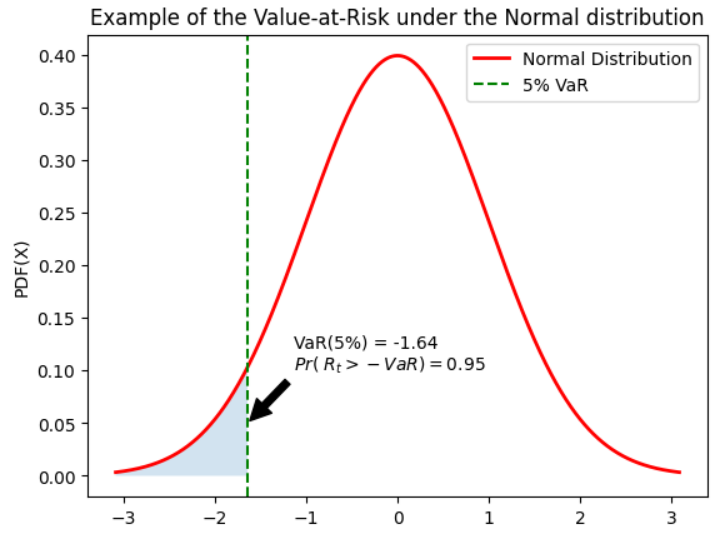
\includegraphics[width = .8\textwidth] {static/course_3_img/VAR_normal.PNG}
\end{frame}

\begin{frame}{VaR: Formal Definition}
\small
\begin{block}{Definition}
    For a hedge rate of $\alpha$\%, the Value-at-Risk, noted $VaR_t (\alpha)$, corresponds to the opposite of the fractile of order $\alpha$ of the distribution of profits and losses (P\&L) 
    $$VaR_t(\alpha) = -F^{-1}_{R_t}(\alpha)$$
    where $F_{R_t}$ denotes the cumulative distribution function associated with the density function $f_{R_t}(.)$
\end{block}
\begin{itemize}
    \item Sometimes the Value-at-Risk is expressed as a function of confidence level. VaR at hedge rate 1\% will be Var(99\%)
    $$VaR(1-\alpha) = -F_{R_t}^{-1}(\alpha)$$
    \item the probability of observing a loss greater than the VaR over the holding period is equal by definition to the coverage rate:
    $$Pr[R_t>-VaR_t(\alpha)] = \int_{-\infty}^{-VaR_t(\alpha)}{f_{R_t}(r) dr} = \alpha $$
\end{itemize}
\end{frame}

\begin{frame}{VaR: Specification}
    The definition of Value-at-Risk is based on 3 elements
\begin{enumerate}
    \item The distribution of profit and loss (P\&L) of the portfolio or the asset
    \item Level of confidence (or equivalently the hedge rate $\alpha$)
    \item The holding period of the asset (or the risk horizon) 
\end{enumerate}
\end{frame}

\begin{frame}{Limites of the Value-at-Risk}
   \centering
   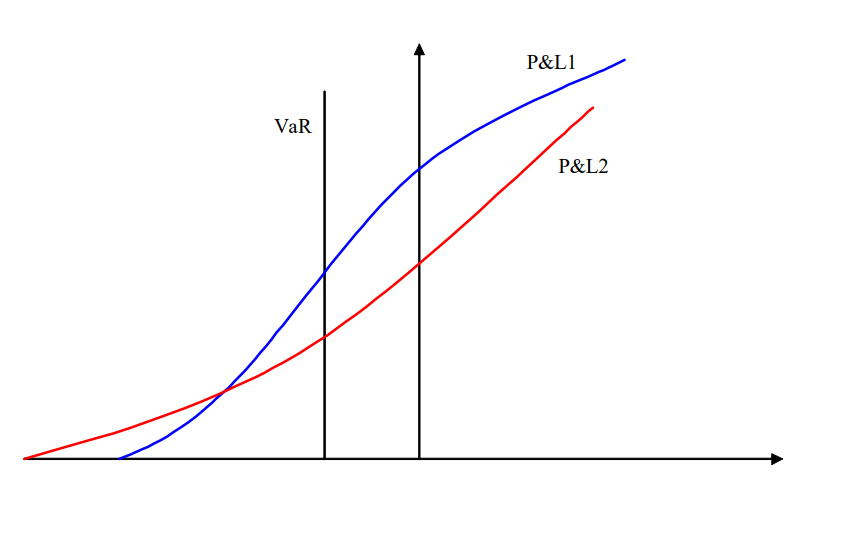
\includegraphics[width=\textwidth]{static/course_3_img/VAR_tail_risk.PNG}
   \begin{enumerate}
       \item This risk measure does not give any information on losses beyond the VaR
   \end{enumerate} 
\end{frame}

\begin{frame}{Limites of the Value-at-Risk}
   \begin{enumerate}
       \item This risk measure does not give any information on losses beyond the VaR
       \item  This measure can lead some agents to voluntarily take more risk in a decentralized risk management system
       \item It can lead to a decision maker to choose a project with exorbitantly  large losses, as long as these losses do not affect the VaR (because they occur with low probability)
       \item the VaR is not a \imfbold{coherent measure of risk} because the \imfbold{sub-additivity} property is not respected
       $$\rho(X+Y) \leq \rho(X) + \rho(Y)$$
   \end{enumerate} 
\end{frame}
\begin{frame}{Expected Shortfall}
    \begin{block}{ES: Expected shortfall}
        The Expected shortfall (ES) associated with a hedge rate $\alpha$ is the average of the $\alpha$\% worst expected losses 
        $$ES_t(\alpha) = -\frac{1}{\alpha} \int_0^{\alpha}{F_{R_t}^{-1}(p)dp} $$
        where $F_{R_t}$ is the cumulative distribution of the density function $f_{R_t}(r)$
    \end{block}
    \begin{itemize}
        \item \textbf{Remark 1: The Expected Shortfall is sometimes denoted the \imfbold{Conditional Loss} or \imfbold{Expected Tail Loss}}
        \item The ES gives average loss in the worst case scenario. i.e in the $\alpha$\% situations where the losses exceed the Var
    \end{itemize}
\end{frame}

\begin{frame}{Expected Shortfall}
   \centering
   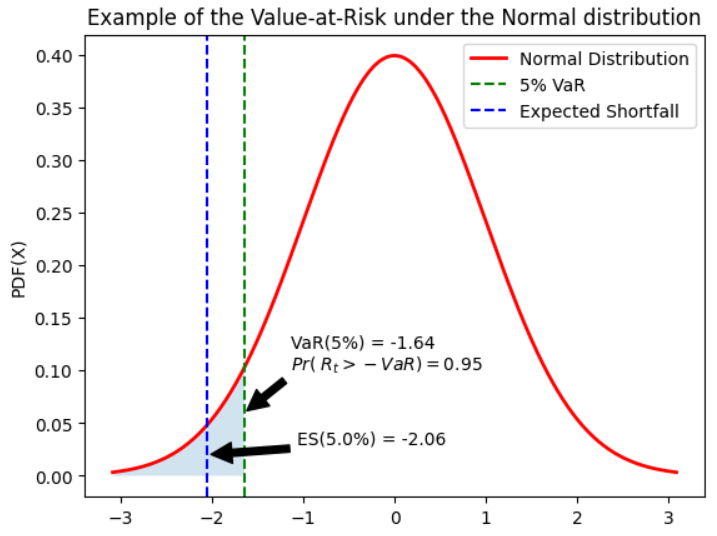
\includegraphics[width=.9\textwidth]{static/course_3_img/ES_normal.PNG}
\end{frame}
\begin{frame}
    \centering
    \Huge Thank you for your attention!
\end{frame}

\appendix
\begin{frame}{Property 1: \emph{Proof}}
    Consider the following ARCH process
    \begin{align*}
        X_t & = Z_t\sigma_t\\
        \sigma_t^2 &= \alpha_0 +\alpha_1X_{t-1}^2
    \end{align*}
    Add $X_t^2$ on both sides of the second equation and rearrange, we get
    \begin{align*}
        X_t^2 &= \alpha_0 +\alpha_1X_{t-1}^2 + (X_t^2 - \sigma_t^2)\\
              &= \alpha_0 +\alpha_1X_{t-1}^2 + (Z_t^2\sigma_t^2 - \sigma_t^2)\\  
              & = \alpha_0 +\alpha_1X_{t-1}^2 + \sigma_t^2(Z_t^2 - 1)\\   
    \end{align*}
    $\nu_t= X_t^2 - \sigma_t^2 = \sigma_t^2(Z_t^2 - 1)$ is an innovation, i.e $\Esp[\nu_t|\underline{X}_{t-1}]=0$
    \begin{align*}
        \Esp[\nu_t|\underline{X}_{t-1}] &= \Esp[\sigma_t^2(Z_t^2 - 1)|\underline{X}_{t-1}]\\
                                        &= \sigma_t^2 \Esp[(Z_t^2 - 1)|\underline{X}_{t-1}]\\
                                        &= \sigma_t^2 ( \Esp[Z_t^2|\underline{X}_{t-1}]-1)\\
                                        &= \sigma_t^2 (\Var(Z_t) - 1)  = 0
    \end{align*}
\end{frame}

\begin{frame}{Property 2: \emph{Proof}}
    Consider the following ARCH process
    \begin{align*}
        X_t & = Z_t\sigma_t\\
        \sigma_t^2 &= \alpha_0 +\alpha_1X_{t-1}^2
    \end{align*}
    $X_t$ is a martingale di§erence, since
    \begin{align*}
        \Esp[X_t|\underline{X}_{t-1}] &= \Esp[Z_t\sigma_t|\underline{X}_{t-1}]\\
                                      &= \sigma_t\Esp[Z_t|\underline{X}_{t-1}]\\
                                      &= \sigma_t\Esp[Z_t]\\
                                      &= 0\\
    \end{align*}
    Since $Z_t$ is an i.i.d process of mean 0
\end{frame}


\begin{frame}{Property 3: \emph{Proof}}
    Consider an ARCH(1) model $X_t$
    \begin{align*}
        \Esp(X_t) &= \Esp(Z_t\sigma_t)\\
                  &= \Esp[\Esp(Z_t\sigma_t|\underline{X}_{t-1})]\\
                  &= \Esp[\sigma_t\Esp(Z_t|\underline{X}_{t-1})]\\
                  &= \Esp[\sigma_t\times 0]\\
                  &=0\\
    \end{align*}
    Since $\Esp[X_t]=0$,  we have $\Var(X_t)=\Esp[X_t^2]$
    
    We know that $X_t^2$ has an AR(1) representation with 
    $$ \Esp[X_t^2] = \Esp[\alpha_0 + \alpha_1 X_{t-1}^2 + \nu_t] = \alpha_0 + \alpha_1 \Esp[X_{t-1}^2] $$
    $$ \Leftrightarrow \Esp[X_t^2] =\frac{\alpha_0}{1-\alpha_1} $$
\end{frame}
\begin{frame}{Property 4: \emph{Proof}}
Consider an ARCH(1) model $X_t$, we have
\begin{align*}
    \Esp(X_t^4|\underline{X}_{t-1}) &= \Esp(Z_t^4 \sigma_t^4|\underline{X}_{t-1})\\
                                    &= \Esp(Z_t^4|\underline{X}_{t-1}) \sigma_t^4\\
                                    &= \Esp(Z_t^4) (\sigma_t^2)^2\\
\end{align*}
$Z_t \overset{\mathrm{i.i.d}}{\sim} \N(0,1)$, so $\Esp(Z_t^4) = 3$. We get
$$ \Kurt(X_t^4|\underline{X}_{t-1}) = \frac{\Esp(X_t^4|\underline{X}_{t-1})}{\Var(X_t^4|\underline{X}_{t-1})^2} = \frac{3(\sigma_t^2)^2}{(\sigma_t^2)^2} =3  $$
The conditional distribution is \imfbold{mesokurtic}
\end{frame}

\begin{frame}{Property 4: \emph{Proof (cont'd) }}
\small
\begin{align*}
   \Esp[X_t^4] &= \Esp(\Esp(X_t^4|\underline{X}_{t-1}))\\ 
               &= 3\Esp( (\alpha_0 +\alpha_1X_{t-1}^2)^2 )\\  
               &= 3\left( \alpha_0^2 + 2\alpha_0\alpha_1\Esp(X_{t-1}^2) +\alpha_1^2\Esp(X_{t-1}^4) \right) \\
               &= 3\left( \alpha_0^2 + \frac{2\alpha_0^2\alpha_1}{1-\alpha_1} +\alpha_1^2\Esp(X_{t-1}^4) \right) \\
               &= 3\alpha_0^2 \left(\frac{1+\alpha_1}{1-\alpha_1} \right) + 3\alpha_1^2\Esp(X_{t-1}^4)
\end{align*}
$X_t$ is stationary, then $\Esp[X_t^4] =\Esp[X_{t-1}^4]$, and we know $\Var(X_t) = \frac{\alpha_0}{(1-\alpha_1)}$
$$ \Esp[X_t^4] =\frac{3\alpha_0^2(1+\alpha_1)}{(1-3\alpha_1^2)(1-\alpha_1) )}$$
$$\Kurt(X_t) = \frac{\Esp(X_t^4}{\Var(X_t)^2} = \frac{3\alpha_0^2(1+\alpha_1)}{(1-3\alpha_1^2)(1-\alpha_1) )} \frac{\alpha_0}{(1-\alpha_1)} = 3 \left( \frac{1-\alpha_1^2}{1-3\alpha_1^2} \right) > 3$$
The Kurtosis is finite and positive as soon as $\alpha_1^2<1/3$. Moreover, the conditional distribution is \imfbold{leptokurtic}.
\end{frame}

\begin{frame}{Conditional Value-at-Risk}
\small
\begin{itemize}
    \item We define the conditional distribution of P\&L, based on a \textbf{set of information available at time t}, denoted as $\Omega_t$
     $$f_{R_t}(r|\Omega_t)$$
     \item the conditional distribution may change through time, but we usually consider the case of invariant conditional density (given the explanatory variables)
     $$F_{R_t}(r|\Omega) = F_{R}(r|\Omega) \quad \forall t$$
\end{itemize}  
\begin{block}{Definition}
    For a hedge rate of $\alpha$\%, the conditional Value-at-Risk to a set of information $\Omega_t$, noted $VaR_t (\alpha|\Omega_t)$, equals to the opposite of the fractile of order $\alpha$ of the P\&L conditional distribution
    $$VaR_t(\alpha|\Omega_t) = -F^{-1}_{R_t}(\alpha|\Omega_t)$$
    where $F_{R_t}(r|\Omega_t)$ is the cumulative distribution function associated with the conditional density function $f_{R_t}(r|\Omega_t))$
\end{block}
\end{frame}

\begin{frame}{Estimation methods}
\small
\begin{block}{Challenge}
    Theoretically, at each date t, the return $R_t$ is a random variable admitting a distribution $f_{R_t}(.)$ and a fractile $\alpha$. However, we have only one observation $r_t$ of this distribution. From this single realization, \textbf{without any additional hypothesis}, it is impossible to estimate the quantiles of the distribution $f_{R_t}(.)$ at date t, i.e. the VaR
\end{block}
\pause
Several estimation methods have been proposed
    \begin{itemize}
        \item \imfbold{Non-parametric Estimation}: No parametric distribution of P\&L is imposed a priori.
        \imfbold{Historical Simulation}(HS), \textbf{Weighted HS}, \textbf{Filtered HS}
        \item \imfbold{Semi-parametric Estimation}: CAViaR method, Extreme Values Theory
        \item \imfbold{Parametric Estimation}: ARCH, GARCH RiskMetrics
    \end{itemize}
\end{frame}

\begin{frame}{Non-Parametric Estimation}
\small
 \textbf{Historical Simulation}: VaR is estimated as the empirical fractile of past returns
 In the HS approach, we explicitly make 2 strong hypothesis
 \begin{enumerate}
     \item the non-conditional distribution of returns is the same $\forall~t$
     $$f_{R_t}(w) = f_{R}(w)$$
     Consequently, the fractiles of this non-conditional distribution is also the same 
     $$VaR_t(\alpha) = VaR(\alpha)$$
     \item Returns $\{R_1, R_2, ..,R_T\}$ are independent 
 \end{enumerate}        
 $\Rightarrow$ VaR estimated by HS are unconditional, relatively invariant to changes in the economic environment
    \begin{itemize}
        \item compute Var on a \imfbold{rolling window} to introduce a minimum conditioning by deleting very ancient observations
        \item \imfbold{Window size is key}: too small and the estimator is volatile, too large and the estimator is invariant
    \end{itemize}
\end{frame}

\begin{frame}{Non-Parametric Estimation}
    \begin{itemize}
        \item \textbf{Bootstrapped Historical Simulation}: The BHS estimator of the VaR corresponds to the empirical average of VaR-HS obtained from S samples of bootstrapped returns:
        $$\hat{VaR}(\alpha) = \frac{1}{S}\sum_{s=1}^{S} \hat{VaR}_s(\alpha) $$
        
        \item Non-parametric estimation of the density function using for instance \textbf{kernel estimate}
        $$\hat{f}_{R_t}(r_0) = \frac{1}{T\lambda} \sum_{t=1}^T{K\left(\frac{r_t-r_0}{\lambda} \right)}$$
        kernel estimators present edge effects. Their precision is low on the "edges" of the sample, precisely where we want to estimate the VaR
        
        \item \textbf{Weighted Hs} or Hybrid Method: \textbf{Aged-weighted HS} or \textbf{Volatility-weighted HS} 
    \end{itemize}
\end{frame}
\begin{frame}{Semi-Parametric Estimation}
    \imfbold{Quantile Regression and CAViaR}
    \begin{itemize}
        \item \textbf{Motivation:} Instead of modeling the distribution function of returns in the perspective of  calculating its quantiles. Why not model the quantiles directly  
        \item CAViaR for \textbf{Conditional Autoregressive Value at Risk}, by Engle and Manganelli, specify an autoregressive dynamic for conditional quantiles
    \end{itemize}
    

    \begin{block}{CAViaR}
        CAViaR is a model specifed on the fractile. The conditional VaR at hedge rate $\alpha$ is given by 
        \begin{align*}
          VaR_{t|t-1}(\alpha) = \beta_0 + \beta_1VaR_{t-1|t-2}(\alpha) +\\ \beta_2 max(r_{t-1},0) - \beta_3 min(r_{t-1},0)   
        \end{align*}
        
        where $\beta_i \in\R$ 
    \end{block}
\end{frame}

\begin{frame}{Parametric Estimation}
\imfbold{Motivation} For any elliptical distribution, the VaR forecast is a linear transformation of the variance (volatility) forecast. Predicting the variance allows to predict the VaR
\medskip

    \begin{block}{Garch Model}
        Under the normal distribution hypothesis of conditional P\&L, the VaR forecast for hedge rate $\alpha$ is given by 
        $$VaR_{t+1|t}(\alpha) = -\mu-\sqrt{h_{t+1}}\Phi^{-1}(\alpha)$$
        where $h_{t+1}$ is the conditional variance of returns derived from the GARCH model
    \end{block}    
\end{frame}

\begin{frame}{Parametric Estimation}
\begin{block}{RiskMetrics}
    Developed by JP Morgan in the 90s. The forecasted conditional VaR for the hedge rate $\alpha$ is
        $$VaR_{t+1|t}(\alpha) = -\mu-h_{t}\Phi^{-1}(\alpha)$$
    where $\mu$ is the expected return and $h_t$ is the conditional variance
    $$h_t = \lambda h_{t-1}+(1-\lambda)r^2_{t-1}$$
    
    where $\lambda$ is a decay parameter (generally fixed to 0.97)
    \end{block}
    \begin{itemize}
        \item The conditional variance in RiskMetrics follows a \textbf{EWMA (Exponential Weighted Moving Average)} type process: The forecasted variance is a linear function of past innovations and past variance
        \item RiskMetricss  is a special case of GARCH
    \end{itemize}
\end{frame}

\end{document}